\documentclass[border=6pt]{standalone}
\usepackage{tikz}
\usetikzlibrary{arrows.meta,positioning,shapes.geometric,calc}
\begin{document}
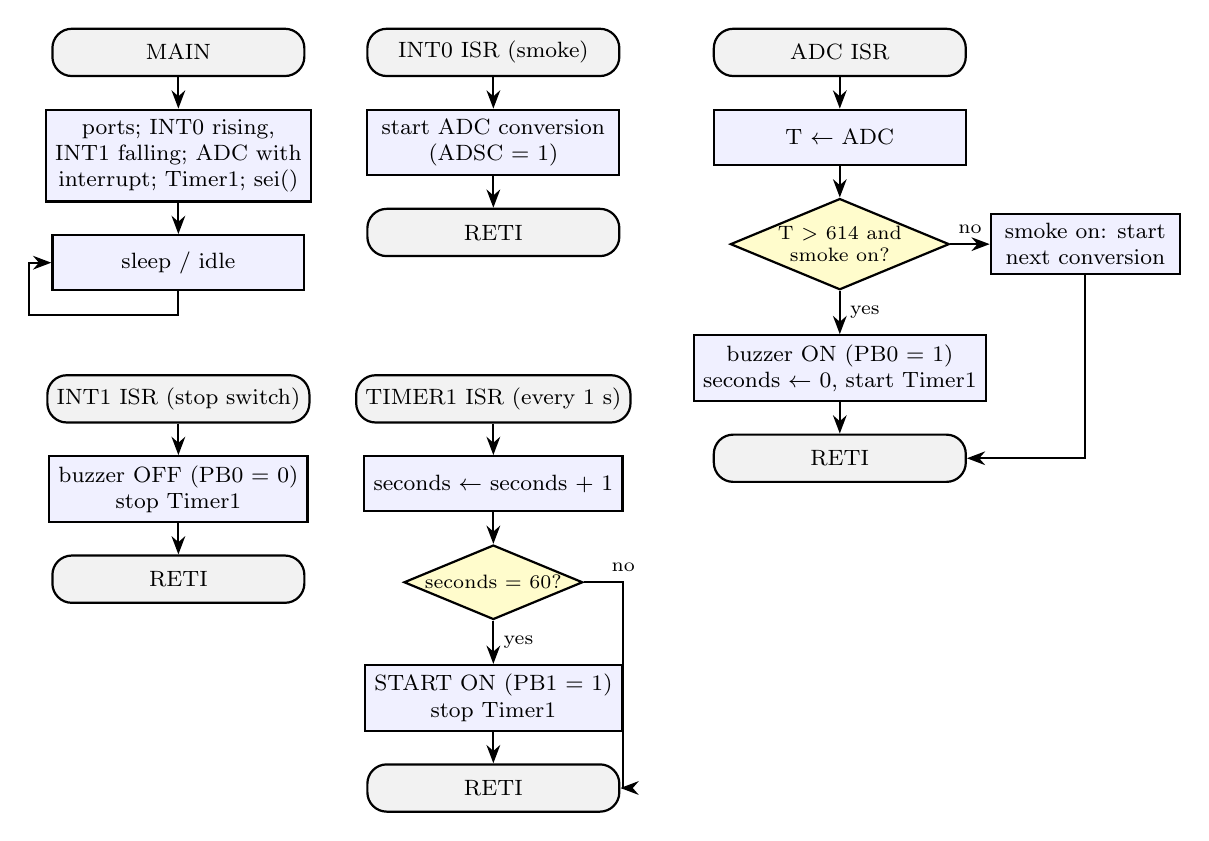
\begin{tikzpicture}[>=Stealth,font=\small,node distance=0.4cm,
 term/.style={draw,thick,rounded corners=7pt,fill=gray!10,minimum width=3.2cm,minimum height=0.6cm,align=center,font=\footnotesize},
 proc/.style={draw,thick,fill=blue!6,minimum width=3.2cm,minimum height=0.7cm,align=center,font=\footnotesize},
 dec/.style={draw,thick,diamond,aspect=2.4,fill=yellow!20,align=center,font=\scriptsize,inner sep=0.5pt}]
% MAIN
\node[term] (m0) {MAIN};
\node[proc,below=of m0] (m1) {ports; INT0 rising,\\INT1 falling; ADC with\\interrupt; Timer1; sei()};
\node[proc,below=of m1] (m2) {sleep / idle};
\draw[->,thick] (m0) -- (m1); \draw[->,thick] (m1) -- (m2);
\draw[->,thick] (m2.south) -- ++(0,-0.3) -- ++(-1.9,0) |- (m2.west);
% INT0
\begin{scope}[xshift=4.0cm]
\node[term] (a0) {INT0 ISR (smoke)};
\node[proc,below=of a0] (a1) {start ADC conversion\\(ADSC = 1)};
\node[term,below=of a1] (a2) {RETI};
\draw[->,thick] (a0) -- (a1); \draw[->,thick] (a1) -- (a2);
\end{scope}
% ADC
\begin{scope}[xshift=8.4cm]
\node[term] (b0) {ADC ISR};
\node[proc,below=of b0] (b1) {T $\leftarrow$ ADC};
\node[dec,below=of b1] (b2) {T $>$ 614 and\\smoke on?};
\node[proc,below=0.55cm of b2] (b3) {buzzer ON (PB0 = 1)\\seconds $\leftarrow$ 0, start Timer1};
\node[term,below=of b3] (b4) {RETI};
\node[proc,right=0.5cm of b2,minimum width=2.4cm] (b5) {smoke on: start\\next conversion};
\draw[->,thick] (b0) -- (b1); \draw[->,thick] (b1) -- (b2);
\draw[->,thick] (b2) -- (b3) node[midway,right,font=\scriptsize]{yes};
\draw[->,thick] (b3) -- (b4);
\draw[->,thick] (b2) -- (b5) node[midway,above,font=\scriptsize]{no};
\draw[->,thick] (b5) |- (b4);
\end{scope}
% INT1
\begin{scope}[yshift=-4.4cm]
\node[term] (c0) {INT1 ISR (stop switch)};
\node[proc,below=of c0] (c1) {buzzer OFF (PB0 = 0)\\stop Timer1};
\node[term,below=of c1] (c2) {RETI};
\draw[->,thick] (c0) -- (c1); \draw[->,thick] (c1) -- (c2);
\end{scope}
% TIMER1
\begin{scope}[xshift=4.0cm,yshift=-4.4cm]
\node[term] (d0) {TIMER1 ISR (every 1 s)};
\node[proc,below=of d0] (d1) {seconds $\leftarrow$ seconds + 1};
\node[dec,below=of d1] (d2) {seconds = 60?};
\node[proc,below=0.55cm of d2] (d3) {START ON (PB1 = 1)\\stop Timer1};
\node[term,below=of d3] (d4) {RETI};
\draw[->,thick] (d0) -- (d1); \draw[->,thick] (d1) -- (d2);
\draw[->,thick] (d2) -- (d3) node[midway,right,font=\scriptsize]{yes};
\draw[->,thick] (d3) -- (d4);
\draw[->,thick] (d2.east) -- ++(0.5,0) node[above,font=\scriptsize]{no} |- (d4.east);
\end{scope}
\end{tikzpicture}
\end{document}
